
\part{Transmutation of Differential Operators}\label{part1} %part 1

\chapter{Riemann's Method}\label{part1:chap1} %chap 1

\section{Riemann's Method for the Cauchy problem}\label{part1:chap1:sec1}

\begin{defi*}
  A\pageoriginale function is said to be $(C,r)$ on a subset of $A$ of $R^n$ if all
  its partial derivatives upto the order $r$ exists and are continuous
  in $A$. 
\end{defi*}

Let $D$ be a region (open connected set) in $R^2$, the $(x,y)$
plane. Let $a,b,c$ be three functions which are $(C,1)$ in $D$ and $u$
a function $(C, 2)$ in $D$ and let $L$ denote the differential
operator 
$$
Lu=\frac{\partial^2 u}{\partial x \partial y} + a \frac{\partial
  u}{\partial x} + b \frac{\partial u}{\partial y} + cu. 
$$
Let $v$ be a function which is $(C, 2)$ in $D$ and $L^*$ be a
differential operator of the same type as $L$: 
$$
L^* v = \frac{\partial^2 v}{\partial x \partial y}-
\frac{\partial}{\partial x }(av) - \frac{\partial}{\partial y}(bv) +cv 
$$
then
\begin{equation}
vL(u) - uL^*(v) = \frac{\partial M}{\partial x}+ \frac{\partial
  N}{\partial y} \tag{1}\label{part1:chap1:sec1:eq1} 
\end{equation}
where\pageoriginale $M$ and $N$ are $(C, 1)$ in $D$ and are certain combinations of
$u, v$ and their partial derivatives. 
\begin{align*}
  v L(u) & = v \frac{\partial^2 v}{\partial x \partial y} + av
  \frac{\partial u}{\partial x}+bv \frac{\partial u}{\partial y} + cuv \\
  & = cuv + \frac{\partial }{\partial x}(auv) +
  \frac{\partial}{\partial y} (buv) + \frac{\partial}{\partial x} \left(v
  \frac{\partial u}{\partial y}\right)\\ 
  & \hspace{2cm}-u  \frac{\partial }{\partial x}(av) -u \frac{\partial}{\partial
    y} (bv) - \frac{\partial v}{\partial x} \frac{\partial u}{\partial
    y}\\ 
  & = u \left[ \frac{\partial^2 v}{\partial x \partial y}-
    \frac{\partial}{\partial x} (av) - \frac{\partial}{\partial
      y}(bv)+cv \right ]\\ 
  &  \hspace{2cm}+ \frac{\partial }{\partial x}\left [auv + v \frac{\partial
      u}{\partial y}\right ] -\frac{\partial}{\partial y}\left [ u
    \frac{\partial v}{\partial x}- buv \right] 
\end{align*}
\begin{align*}
 vL(u)-uL^* (v) & = \frac{\partial M}{\partial x}+\frac{\partial
    N}{\partial y} \qquad \text{ where }\\ 
 M & = auv + v \frac{\partial u}{\partial y}, N = buv - u \frac{\partial
  v}{\partial x}. 
\end{align*}

The right hand member of (\ref{part1:chap1:sec1:eq1}) does not change
if we replace $M$ by 
$auv +\dfrac{1}{2}(v \dfrac{\partial u}{\partial y}-u \dfrac{\partial
  v}{\partial y})$ and $N$ by $buv +\dfrac{1}{2}(v \dfrac{\partial
  u}{\partial x}-u \dfrac{\partial v}{\partial x})$. We prefer to have 
\begin{align*}
  M=\frac{1}{2} \frac{\partial}{\partial y}(uv)-u P(v)
  \tag{i}\label{part1:chap1:sec1:eqi} \\
  N=\frac{1}{2} \frac{\partial}{\partial x}(uv)-u Q(v)
  \tag{ii}\label{part1:chap1:sec1:eqii} 
\end{align*}
where 
$$
P(v) = \frac{\partial v}{\partial y}- av~, Q(v)= \frac{\partial
  v}{\partial x} - bv. 
$$

Let\pageoriginale $C$ be a closed curve lying entirely in the region $D$.

By Green's formula,

$$
\int_C (\lambda M + \mu N) ds = \int \int_A \left(\frac{\partial
  M}{\partial x} + \frac{\partial N}{\partial y}\right)~ dxdy 
$$
where $\lambda$, $\mu$ denote the direction cosines of the interior
normal to $C$ and $A$ denotes the region enclosed by $C$. 

In view of equation (\ref{part1:chap1:sec1:eq1}),
\begin{equation}
  \int_C (\lambda M + \mu N) ds = \int \int_A (v L(u) - u L^* (v))
  dxdy \tag{2}\label{part1:chap1:sec1:eq2} 
\end{equation}

We shall consider this equation in the case when $C$ consists of two
straight lines $AX$, $AY$ parallel to the axes of coordinates and a
curve $\Gamma$, monotonic in the sense of $AX$ and $AY$, joining $X$
and $Y$. Suppose that $L(u)=0$ and $L^* (v) = 0$ then $\int_C (\lambda
M + \mu N)ds =0$ i.e. $\int^X_A Ndx - \int^A_Y M dy = \int ^X_Y
(\lambda M + \mu N)ds$ substituting for $M$ and $N$ from
(\ref{part1:chap1:sec1:eqi}) and (\ref{part1:chap1:sec1:eqii}) respectively, 
\begin{figure}[H]
  \centering{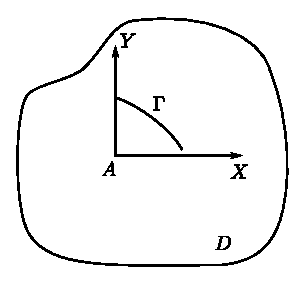
\includegraphics{vol22-figures/fig22-1.eps}}
\end{figure}
$$
\displaylines{\hfill 
  \int \limits^X_A N dx = \frac{1}{2} \left [ (uv)_X - (uv)_A \right ] -
  \int \limits^X_A u Q(v) dx \hfill\cr 
  \text{and} \hfill 
  -\int^A_Y M dy = \frac{1}{2} \left[ (uv)_Y - (uv)_A \right ] +
  \int^A_Y u P(v) dy. \hfill } 
$$
If\pageoriginale the functions $u,v$ satisfy
\begin{equation*}
  Lu = 0, L^* v = 0, P(v)= 0 \text{ on } AY \text{ and } Q(v) = 0
  \text{ on } AX \tag{3}\label{part1:chap1:sec1:eq3} 
\end{equation*}
then we obtain the Riemann's Resolution formula:
$$
(uv)_A = \frac{1}{2}\left[(uv)_X + (uv)_Y \right]+ \int ^X_Y (\lambda
M + \mu N) ds. 
$$
Let $A$ be $(x_0, y_0)$. Then $v=g(x,y ; x_0, y_0)$ satisfying the
conditions (\ref{part1:chap1:sec1:eq3}) is the Riemann's function
for the equation $L(u)=0$.  

In the situation
$$
L(u) = f(x,y), L^* v = 0, P(v)=0 \text{ on } AY, Q(v) = 0 \text{ on }
AX, 
$$
exactly similar computation gives the formula:
\begin{gather*}
  (uv)_A = \frac{1}{2} \left [ (uv)_X + (uv)_Y \right ]+ \int ^X_Y
  (\lambda M + \mu N) ds 
  + \int \int_A vf(x,y) dxdy.
\end{gather*}

\heading{An important property of the Riemann's function.}

Let now $\Gamma$ consider of two straight lines $XB, YB$ parallel to
the axes of coordinates. Then 
$$
\int^X_Y (\lambda M + \mu N) ds = \int^X_B M dy -  \int^B _Y N dx
$$
\begin{align*}
  \text{ We can write } \hspace{1cm}M & = - \frac{1}{2} \frac{\partial}{\partial
    y} (uv) + v P^* (u)\hspace{3cm} \\ 
  N & = - \frac{1}{2} \frac{\partial}{\partial x}(uv) + v Q^*(u)
\end{align*}
where\pageoriginale $P^* (u) = \dfrac{\partial u}{\partial y}+au~, ~ Q^*(u) =
\dfrac{\partial u}{\partial x}+ bu$. 
\begin{multline*}
  \int^X_B M dy = - \frac{1}{2} \left[(uv)_X - (uv)_B \right] +
  \int^X_B vP^* (u) dx \\ 
  - \int^B_Y N dx = \frac{1}{2} \left[(uv)_B - (uv)_Y \right]-
  \int^B_Y vQ^* (u) dx 
\end{multline*}

Thus in this case Riemann's resolution formula becomes
\begin{align*}
  (uv)_A &=\frac{1}{2} \left [ (uv)_X + (uv)_Y \right] -
  \frac{1}{2}\left [ (uv)_X - (uv)_B \right] \\ 
  & \hspace{.5cm} + \int^X_B v P^* (u)dx + \frac{1}{2} \left [ (uv)_B -
    (uv)_Y \right] - \int^B_Y vQ^* (u) dx\\ 
  \text{i.e.,} ~~  (uv)_A & = (uv)_B - \int^B_Y v Q^* (u)dx +
  \int^X_B v P^* (u) dx 
\end{align*}

If $u=h(x,y ; x_1,y_1), (x_1,y_1)$ being the point $B$, is such that
$$
\displaylines{\hfill 
  Lu = 0, P^*(u) = 0 \text{ on }BX, Q^*(u) = 0 \text{ on }BY,\hfill \cr 
  \text{we get}\hfill  (uv)_A = (uv)_B. \hfill }
$$

Choosing constant multipliers for $u = h(x,y; x_1,y_1)$ and  $v=g$
$(x,y; x_0, y_0)$\pageoriginale in such a way that $u = 1$ at 
$B$ and $v=1$ at $A$, we have  
\begin{equation}
  h(x_0, y_0 ; x_1, y_1) = g(x_1,y_1 ; x_0, y_0)
  \tag{4}\label{part1:chap1:sec1:eq4} 
\end{equation}

This shows that the Riemann's function $g$, considered as a function
of $(x_0, y_0)$ satisfies the differential equation $Lu = 0$. 

\section{Proof for the Riemann's method}\label{part1:chap1:sec2}

We have obtained (\ref{part1:chap1:sec1:eq4}) under the hypothesis that there exists
functions $u=h(x,y ; x_1,y_1)$ and $v=g(x,y ; x_0,y_0)$ which are $(C,
2)$ in $D$ and which satisfy 
\begin{align*}
  Lu & =  \frac{\partial^2 u}{\partial x \partial y}+ a \frac{\partial
    u}{\partial x} + b \frac{\partial u}{ \partial y}+ cu = 0 \\ 
  P^* (u) & = \frac{\partial u}{\partial y}+au = 0 \text{ on }BX \\
  Q^* (u) & = \frac{\partial u}{\partial x}+bu = 0 \text{ on }BY \text{ and } \\
  L^* v & = \frac{\partial^2 v}{\partial x \partial y}+ a^*
  \frac{\partial v}{\partial x}+b^* \frac{\partial v}{\partial y}+c^*
  v = 0 \text{ where } \\
  a^* & = -a, b^* = -b, c^* = - \frac{\partial a}{\partial x} -
  \frac{\partial b}{\partial y}+c 
\end{align*}
\begin{align*}
  P(v) &= \frac{\partial v}{\partial y} + a^* (v) = 0 \text{ on } AY \\
  Q(v) &= \frac{\partial v}{\partial x}+b^* (v) = 0 \text{ on } AX.
\end{align*}

By\pageoriginale change of notation and translation of the origin, the problem for
the existence of the Riemann's function $v=g(x,y)$ in $D$ for the
point $(x_0, y_0) \in D$ for the differential equation $Lu = 0$
reduces to the solution of the problem $1$: 
$$
\frac{\partial^2 u}{\partial x \partial y}+ a \frac{\partial
  u}{\partial x} + b \frac{\partial u}{\partial y} + cu = 0 
$$
with the conditions
\begin{align*}
  u(0,y) & = \alpha(y) \\
  u(x,0) & = \beta(x) ~ I\\
  \alpha(0) & = \beta (0) = 1
\end{align*}
where $a, b, c$ are $(C,1)$ in $D$ and $\alpha,\beta$ are $(C,1)$
functions of one real variable. The solution of the more general
problem \ref{part1:chap1:sec1:eq2}: 
$$
\frac{\partial^2 u}{\partial x \partial y} = \lambda \left [ a
  \frac{\partial u}{\partial x} + b \frac{\partial u}{\partial y} + cu
  \right] 
$$
with the conditions $I$ will give for $\lambda = -1$ the solution of
the problem (\ref{part1:chap1:sec1:eq1}). We shall now prove the existence of the unique
solution for the problem \ref{part1:chap1:sec1:eq2} by using Piccard's method of successive
approximations. Consider the series 
\begin{equation}
  u_0 (x,y) + \lambda u_1 (x,y) + \cdots + \lambda^n u_n (x,y) +
  \cdots \tag{5}\label{part1:chap1:sec2:eq5} 
\end{equation}
where\pageoriginale $u_i (x,y)$ are defined by the following recurrence formula:
\begin{multline*}
  ~\frac{\partial^2 u_0}{\partial x \partial y} = 0~ u_0(0,y) =
  \alpha(y), u_0 (x,0) = \beta(x) \\ 
  \frac{\partial^2 u_n}{\partial x \partial y} = a \frac{\partial
    u_{n-1}}{\partial x} + b \frac{\partial u_{n-1}}{\partial y}+
  cu_{n-1}, u_n(x,0) = u_n(0,y) =0 ~\text{ for } n \geq 1. 
\end{multline*}

It suffices to take $u_0 (x,y) = \alpha(y) + \beta (x) -1$ and $u_n
(x,y) = \int^x_0 \int^y_0$ $\phi_{n-1} (\xi,  \eta) d \xi d \eta$ where 
$$
\phi_{n-1} = a \frac{\partial u_{n-1}}{\partial x} + b \frac{\partial
  u_{n-1}}{\partial y} + cu_{n-1} 
$$
We shall now prove the convergence of the series (\ref{part1:chap1:sec2:eq5}) by the process
of majorisation which is classical. Suppose that $a,b,c$ are $(C,0)$
in $D$ and $\alpha,  \beta$ are $(c,1)$ of one real variable. Let $K$
be a compact subset $D$ containing the rectangle with sides parallel
to the axes and $(0, 0)$ and $(x,y)$ as opposite corners. Then there
exists an $M, A$ such that $| \alpha (\xi) + \beta (\eta)-1 | \leq M$, 
$$
\displaylines{\hfill 
  | \frac{\partial}{\partial \xi}  (\alpha (\xi) + \beta (\eta ) -1) |
  \leq M, \hfill\cr 
  \text{and }\hfill  | \frac{\partial}{\partial \eta}  (\alpha (\xi) +
  \beta (\eta ) -1) | \leq M, \phantom{and}\hfill }
$$
for $(\xi,  \eta)$ in $K$, and $|a|, |b|, |c|, \leq A$ in $K$. Then $|
\phi_0 (x,y) | \leq 3$\pageoriginale A M. By the recurrence formula for $n=1$, 
$$
  | u_1 (x,y) | \leq | \int^x_0 \int^y_0 \phi_0 (\xi, \eta ) d \xi d
   \eta | \leq 3 A M |x|| y |
$$
 $\Bigg| \dfrac{\partial u_1}{\partial x}\Bigg| \leq 3 AM | y |$  and,
  $ \Bigg|\dfrac{\partial u_1}{\partial y}\Bigg| \leq 3 A M | x|$.  Hence 
 $ | u_1 (x,y) |,  \Bigg|\dfrac{\partial u_1}{\partial x}\Bigg|,
   \Bigg|\dfrac{\partial u_1}{\partial y}\Bigg|$ are each  $\leq 3 A M
   (1+ |x|) (1+|y|)$.  

Computing $\phi_1 (x,y)$, we have immediately,  
\begin{align*}
  |u_2 (x,y)| &\leq 9 A^2 M \left(\frac{1+|x|}{2!}\right)^2
  \left(\frac{1+|y|}{2!}\right)^2\\ 
   \left |  \frac{\partial u_2 (x,y)}{\partial x} \right|  &\leq 9 A^2 
  M (1+|x|) \left(\frac{1+|y|}{2}\right)^2 \\ 
   \left | \frac{\partial u_2 (x,y)}{\partial y} \right | &\leq 9 A^2
  M   \left(\frac{1+|x|}{2}\right)^2 (1+|y|)\\
  \intertext{In general} 
  | u_n(x,y)|,  \left | \dfrac{\partial
    u_n}{\partial x} \right |, \left | \dfrac{\partial u_n}{\partial
    y} \right |, & \leq  \dfrac{M [ 3A (1+|x|)(1+|y|)]^n}{n !} 
\end{align*}

 Comparing with the exponential series, this majorization proves that
 the series (\ref{part1:chap1:sec1:eq3}) as also the series obtained from (\ref{part1:chap1:sec1:eq3}) by
 differentiating each term once and twice are all convergent uniformly
 on each compact subset of $D$ and absolutely in $D$, so that
 (\ref{part1:chap1:sec1:eq3})
 converges to a function $(C,2)$ in $D$. This function $u(x,y)$ is
 evidently the solution of problem \ref{part1:chap1:sec1:eq2} and the
 proof for the existence of Riemann's functions is complete. 

\begin{remark*}
  From\pageoriginale the recurrence formula it is clear that the
  function $u(x,y)$ satisfies 
  \begin{multline*}
  u(x,y) = \alpha(y) + \beta (x) -1 + \lambda \int^x_0 \int^y_0 \left[
    a \frac{\partial u}{\partial x} + b \frac{\partial u}{\partial y}+
    cu \right] d \xi ~ d \eta~\\ 
  {\substack{x=\xi\\ y = \eta}}\qquad \quad  
  \end{multline*}
  This integral equation is equivalent to the differential equation of
  problem \ref{part1:chap1:sec1:eq2} with conditions $I$. When $a, b, c$ are $(C, 0)$ and
  $\alpha, \beta$ are $(C, 1)$, the solution $u(x,y)$ of the integral
  equation may not be $(C,2)$. But then it is a solution of problem
  \ref{part1:chap1:sec1:eq2} in the sense of distributions. 
\end{remark*}
